% AUTHOR ===================================================================================================================
% Manuel Lippert (GitHub: ManeLippert (https://github.com/ManeLippert))
% ==========================================================================================================================

% PREAMBLE =================================================================================================================

% ****** Start of file aipsamp.tex ******
%
%   This file is part of the AIP files in the AIP distribution for REVTeX 4.
%   Version 4.1 of REVTeX, October 2009
%
%   Copyright (c) 2009 American Institute of Physics.
%
%   See the AIP README file for restrictions and more information.
%
% TeX'ing this file requires that you have AMS-LaTeX 2.0 installed
% as well as the rest of the prerequisites for REVTeX 4.1
% 
% It also requires running BibTeX. The commands are as follows:
%
%  1)  latex  aipsamp
%  2)  bibtex aipsamp
%  3)  latex  aipsamp
%  4)  latex  aipsamp
%
% Use this file as a source of example code for your aip document.
% Use the file aiptemplate.tex as a template for your document.

% DOCUMENT =================================================================================================================

\documentclass[aip, amsmath, amssymb, reprint, twocolumn, floatfix]{revtex4-1}

% documentclass revtex4-1 options:
% - aip,
% - jmp,
% - bmf,
% - sd,
% - rsi,
% - amsmath,amssymb,
% - preprint,%
% - reprint,%
% - author-year,%
% - author-numerical,%
% - Conference Proceedings

\preprint{AIP/123-QED}

% PACKAGES =================================================================================================================

\usepackage[utf8]{inputenc}
\usepackage[T1]{fontenc}
\usepackage{mathptmx}
\usepackage{etoolbox}
\usepackage{graphicx}% Include figure files
\usepackage{dcolumn}% Align table columns on decimal point
\usepackage{bm}% bold math
%\usepackage[mathlines]{lineno}% Enable numbering of text and display math
%\linenumbers\relax % Commence numbering lines

%% Additional
\usepackage[format=hang]{caption}
\usepackage[hidelinks]{hyperref}

% FUNCTIONS, INPUT =========================================================================================================

\graphicspath{{../pictures/}}% Path for pictures

\newcommand{\wexb}{\omega_{\mathrm{\:E \times B}}}
\newcommand{\hatwexb}{\widehat{\omega}_{\mathrm{\:E \times B}}}
\newcommand{\exb}{\mathrm{\:E}\times\mathrm{B}}
\newcommand{\hatwexbamp}{|\hatwexb|_{\nzf}}
\newcommand{\NR}{N_\mathrm{R}}
\newcommand{\NB}{N_\mathrm{B}}
\newcommand{\rlt}{R/L_T}
\newcommand{\rhoth}{\rho}
\newcommand{\vth}{v_{\mathrm{th}}}
\newcommand{\nzf}{n_\mathrm{ZF}}
\newcommand{\kzf}{k_\mathrm{ZF}}
\newcommand{\xcoord}{x}
\newcommand{\ycoord}{y}

% MAIN =====================================================================================================================

\begin{document}

%% TITLE, INFO =============================================================================================================

\title[Size convergence of the $\exb$ staircase pattern in flux tube simulations of ion temperature gradient-driven turbulence]
{Size convergence of the $\exb$ staircase pattern in flux tube simulations of ion temperature gradient-driven turbulence}

\author{M. Lippert}
	\altaffiliation{Repository of this work: \\ 
					https://github.com/ManeLippert/Bachelorthesis-Shearingrate-Convergence}
\author{F. Rath}
	\altaffiliation{Author to whom correspondence should be addressed: \\
					Florian.Rath@uni-bayreuth.de}
\author{A. G. Peeters}
\affiliation{Physics Department, University of Bayreuth, 95440 Bayreuth, Germany}

\date{\today}

%% ABSTRACT ================================================================================================================

\begin{abstract}
    The radial size convergence of the $\exb$ staircase pattern is addressed in local gradient-driven flux tube simulations of ion temperature gradient (ITG)-driven turbulence.
    Its is shown that a mesoscale pattern size of \linebreak $\sim 57-76\,\rhoth$ is inherent to ITG-driven turbulence with Cyclone Base Case parameters in the local limit. 
    
\end{abstract}
\maketitle

%%% INTRODUCTION ===========================================================================================================

Ion temperature gradient-driven turbulence close to marginal stability exhibits zonal flow pattern formation on mesoscales, so-called $\exb$ staircase structures \cite{Pradalier2010}.
Such pattern formation has been observed in local gradient-driven flux-tube simulations \cite{Peeters2016, Rath2021}, including collisions \cite{Weikl2017} and background $\exb$ shear \cite{Rath2021}, local flux-driven realizations including mean electric field shear \cite{Seiferling2019}, as well as global gradient-driven \cite{McMillan2009, Villard2013, Seo2022} and global flux-driven \cite{Pradalier2010, Pradalier2015, Wang2020, Kim2022, Kishimoto2023} studies. 
In global studies, spanning a larger fraction of the minor radius, multiple radial repetitions of staircase structures are usually observed, with a typical pattern size of several ten Larmor radii.
By contrast, in the aforementioned local studies the radial size of $\exb$ staircase structures is always found to converge to the radial box size of the flux tube domain.
The above observations lead to the question: 
\textit{Does the basic pattern size always converges to the box size, or is there a typical mesoscale size inherent to staircase structures also in a local flux-tube description?}
The latter case would imply that it is not necessarily global physics, i.e., profile effects, that set (i) the radial size of the $\exb$ staircase pattern and (ii) the scale of avalanche-like transport events. These transport events are usually restricted to $\exb$ staircase structures and considered as a nonlocal transport mechanism \cite{Pradalier2010}. 
In this brief communication the above question is addressed through a box size convergence scan of the same cases close to the nonlinear threshold for turbulence generation as studied in Ref.~\onlinecite{Peeters2016}.\bigskip

%%% SIMULATION SET-UP ======================================================================================================

The gyrokinetic simulations are performed with the non-linear flux tube version of Gyrokinetic Workshop (GKW) \cite{Peeters2009} with adiabatic electron approximation.
In agreement with Ref.~\onlinecite{Peeters2016}, Cyclone Base Case (CBC) like parameters are chosen with an inverse background temperature gradient length $\rlt = 6.0$ and circular concentric flux surfaces. 
The numerical resolution is compliant to the "Standard resolution with 6th order (S6)" set-up of the aforementioned reference, with a somewhat lowered number of parallel velocity grid points.
It has been carefully verified that this modification preserves the same physical outcome as the original study.
A summary of the numerical parameters is given in Table~\ref{tab:resolution} and for more details about the definition of individual quantities the reader is referred to Ref.~\onlinecite{Peeters2009, Peeters2016}.
\begin{table}[ht]
	\begin{ruledtabular}
		\begin{tabular}{l | ccccc | ccccc | c | cc}
			& $N_m$ & $N_x$ & $N_s$ & $N_{\nu_\parallel}$ & $N_\mu$ & $D$ & $\nu_d$           & $D_{\nu_\parallel}$ & $D_x$ & $D_y$ & Order & $k_y\rho$ & $k_x\rho$ \\
			\hline
			S6   & 21    & 83    & 16    & 48                  & 9       & 1   & $|\nu_\parallel|$ & 0.2                 & 0.1   & 0.1   & 6     & 1.4       & 2.1       \\
		\end{tabular}
	\end{ruledtabular}
	\caption{
		Resolution used in this paper for further information the author links to Ref.~\onlinecite{Peeters2016}.}
	\label{tab:resolution}
\end{table}

%%% DIAGNOSTICS ================================================================================================================

In the following the box size is increased relative to the standard box size $(L_\xcoord,~L_\ycoord) = (76.3,~89.8)\,\rhoth$ in the radial and binormal direction. Here, $\xcoord$ is the radial coordinate that labels the flux surfaces normalized by the thermal Larmor radius $\rhoth$ and $\ycoord$ labels the field lines and is an approximate binormal coordinate. Together with the coordinate $s$ which parameterizes the length along the field lines and is referred to as the parallel coordinate these quantities form the Hamada coordinates \cite{Hamada1958}.
The increased box sizes are indicated by the real parameter $\NR$ for radial and $\NB$ for the binormal direction with the nomenclature $\NR\times \NB$ throughout this work.
Note that, the number of modes in the respective direction, i.e., $N_x$ and $N_m$, respectively, is always adapted accordingly to retain a spatial resolution compliant to the standard resolution [Table~\ref{tab:resolution}] and standard box size. \\
The $\exb$ staircase pattern is manifest as radial structure formation in the $\exb$ shearing rate defined as\cite{Rath2016, Pueschel2008, Rath2016, Peeters2016}
\begin{equation}
	\wexb = \frac{1}{2} \frac{\partial^2 \langle \phi \rangle}{\partial \xcoord^2}~,
	\label{eq:shearingrate}
\end{equation}
where $\langle \phi \rangle$ is the zonal electrostatic potential normalized by $\rho_\ast T/e$ ($\rho_\ast = \rhoth/R$ is the thermal Larmor radius normalized with the major radius $R$, $T$ is the temperature and $e$ is the elementary charge).
The zonal potential is calculated from the electrostatic potential $\phi$ on the two-dimensional $\xcoord$-$\ycoord$-plane at the low field side according to Ref.~\onlinecite{Rath2021}
\begin{equation}
\langle \phi \rangle = \frac{1}{L_\ycoord} \int_0^{L_\ycoord} \mathrm{d}\ycoord ~ \phi(\xcoord,\ycoord,s=0)~.
\end{equation}
The $\exb$ shearing rate $\wexb$ is the radial derivative of the advecting zonal flow velocity \cite{Hahm1995, Waltz1998} and quantifies the zonal flow induced shearing of turbulent structures \cite{Biglari1990, Hahm1995, Burnell1997}. \\
Consistent with Ref.~\onlinecite{Peeters2016} the turbulence level is quantified by the turbulent heat conduction coefficient $\chi$, which is normalized by $\rhoth^2 \vth/R$ ($\vth = \sqrt{2 T/m}$ is the thermal velocity and $m$ is the mass). Furthermore, quantities $\rhoth$, $R$, $T$, $\vth$ and $m$ are referenced quantities from Ref. \onlinecite{Peeters2016,Peeters2009}.
\newpage
In order to diagnose the temporal evolution of the staircase pattern and to obtain an estimate of its amplitude the radial Fourier transform of the $\exb$ shearing rate is considered. 
It is defined by
\begin{equation}
	\wexb = \sum_{\kzf} \hatwexb(\kzf,t) \, \exp(\mathrm{i} \kzf \xcoord)~,
	\label{eq:shearingrate_fourier}
\end{equation}
where $\hatwexb$ is the complex Fourier coefficient and \linebreak $\kzf = 2\pi \nzf/L_\xcoord$
defines the zonal flow wave vector with the zonal flow mode number $\nzf$ ranging in $-(N_\xcoord -1)/2 \leq \nzf \leq (N_\xcoord -1)/2 $.
Based on the definitions above, the shear carried by the zonal flow mode with wave vector $\kzf$ is defined by $\hatwexbamp = 2 |\hatwexb(\kzf,t)|$. 
In general, the zonal flow mode that dominates the $\exb$ staircase pattern, also referred to as the \textit{basic mode} of the pattern in this work, exhibits the maximum amplitude in the spectrum $\hatwexbamp$.\bigskip

%%% RESULTS ================================================================================================================

In the first test the radial box size is increased while the binormal box size is kept fixed to the standard size. The scan covers the realizations $\NR\times\NB \in [ 1\times1,~2\times1,~3\times1,~4\times1]$.
Each realization exhibits an initial quasi-stationary turbulent phase and a second final \cite{Peeters2016} phase with almost suppressed turbulence [Fig.~\ref{fig:wexb-eflux-1-2-3-4x1-comparison}(a)].
The latter state is indicative for the presence of a fully developed staircase pattern as depicted in Fig.~\ref{fig:wexb-stable-comparison}. 
This type of structure is characterized by intervals of almost constant shear with alternating sign satisfying the Waltz criterion $|\wexb| \approx \gamma$\cite{Waltz1994, Waltz1998} [$\gamma$ is the growth rate of the most unstable linear ion temperature gradient (ITG)-driven Eigenmode], connected by steep flanks where $\wexb$ crosses zero.
The negative gradient of the perturbed perpendicular and parallel ion pressure (not shown) exhibit positive corrugations in regions with maximum $|\wexb|$ and negative corrugations at zero crossings of $\wexb$. 
A radial force balance analysis suggests that the structures in $\wexb$ as depicted in Fig.~\ref{fig:wexb-stable-comparison} are not a consequence of the pressure gradient corrugations as discussed elsewhere \cite{Kosuga2013}.
Rather, the corrugations in the pressure gradient have to be interpreted as a consequence of the staircase structure in $\wexb$ due to the stabilizing zonal flow - turbulence interaction.
Figure~\ref{fig:wexb-stable-comparison}(a) shows a striking repetition of the staircase structure, with the number of repetitions equal to $\NR$.
Hence, the basic size of the pattern not only converges with increasing radial box size, but the converged radial size also turns out to at least roughly agree with the standard radial box size of Ref.~\onlinecite{Peeters2016}.
Due to the lack of a substantial turbulent drive in the final suppressed state no further zonal flow evolution is observed [Fig.~\ref{fig:wexb-eflux-1-2-3-4x1-comparison}(b)] and one might critically ask whether the structures shown in Fig.~\ref{fig:wexb-stable-comparison} represent the real converged pattern in a statistical sense. 
Note that in the $3 \times 1$ case the initial quasi-stationary turbulent state extends up to a few $\sim 10^4\,R/\vth$.
During this period the zonal flow mode with $\nzf = 3$, i.e., the mode that dominates the staircase pattern in final suppressed phase, undergoes a long-term evolution with a typical timescale of several $\sim 10^3\,R/\vth$. 
Hence, several of such cycles are covered by the initial turbulent phase, which is evident from the occurrence of phases with reduced amplitude around $t \approx 8000\,R/\vth$ and $t \approx 18000\,R/\vth$.
It is the $\nzf = 4$ zonal flow mode, i.e., the next shorter radial scale mode, that dominates the shear spectrum $\hatwexbamp$ in the latter two phases (not shown). This demonstrates a competition between the $\nzf = 3$ and $\nzf = 4$ modes.
Most importantly, no secular growth of the $\nzf = 1$ (box scale) zonal flow mode is observed during the entire quasi-stationary turbulent phase [Fig.~\ref{fig:wexb-eflux-1-2-3-4x1-comparison}(b) dotted line].
The above discussion indicates that although the $\nzf = 3,~4$ zonal modes compete, the pattern scale does not converge to the radial box scale but rather to a mesoscale of $\sim 57 - 76\,\rhoth$ (i.e., $\nzf = 4,~3$ in the $3\times1$ case). \bigskip

Since the radially elongated simulation domain might inhibit the development of isotropic turbulent structures, in the second test the radial and binormal box size is increased simultaneously.
This scan covers the realizations $\NR\times\NB \in [1\times1,~1.5\times1.5,~2\times2,~2.5\times2.5,~3\times3]$. Interestingly, suppression of the turbulence by the emergence of a fully developed staircase pattern almost always occurs after $\sim 1000\,R/\vth$ [Fig. \ref{fig:eflux-1x1-2x2-3x3-comparison}], i.e., significantly faster compared to the $3\times1$ and $4\times1$ realizations. As shown in Fig.~\ref{fig:wexb-stable-comparison}(b) this test also confirms the convergence of the staircase pattern size to a typical mesoscale that is distinct from the radial box size in the $\NR > 1$ realizations.

%% Include graphic for two column with specific place
\onecolumngrid
\begin{center}
	\centering
	\captionsetup{type=figure}
	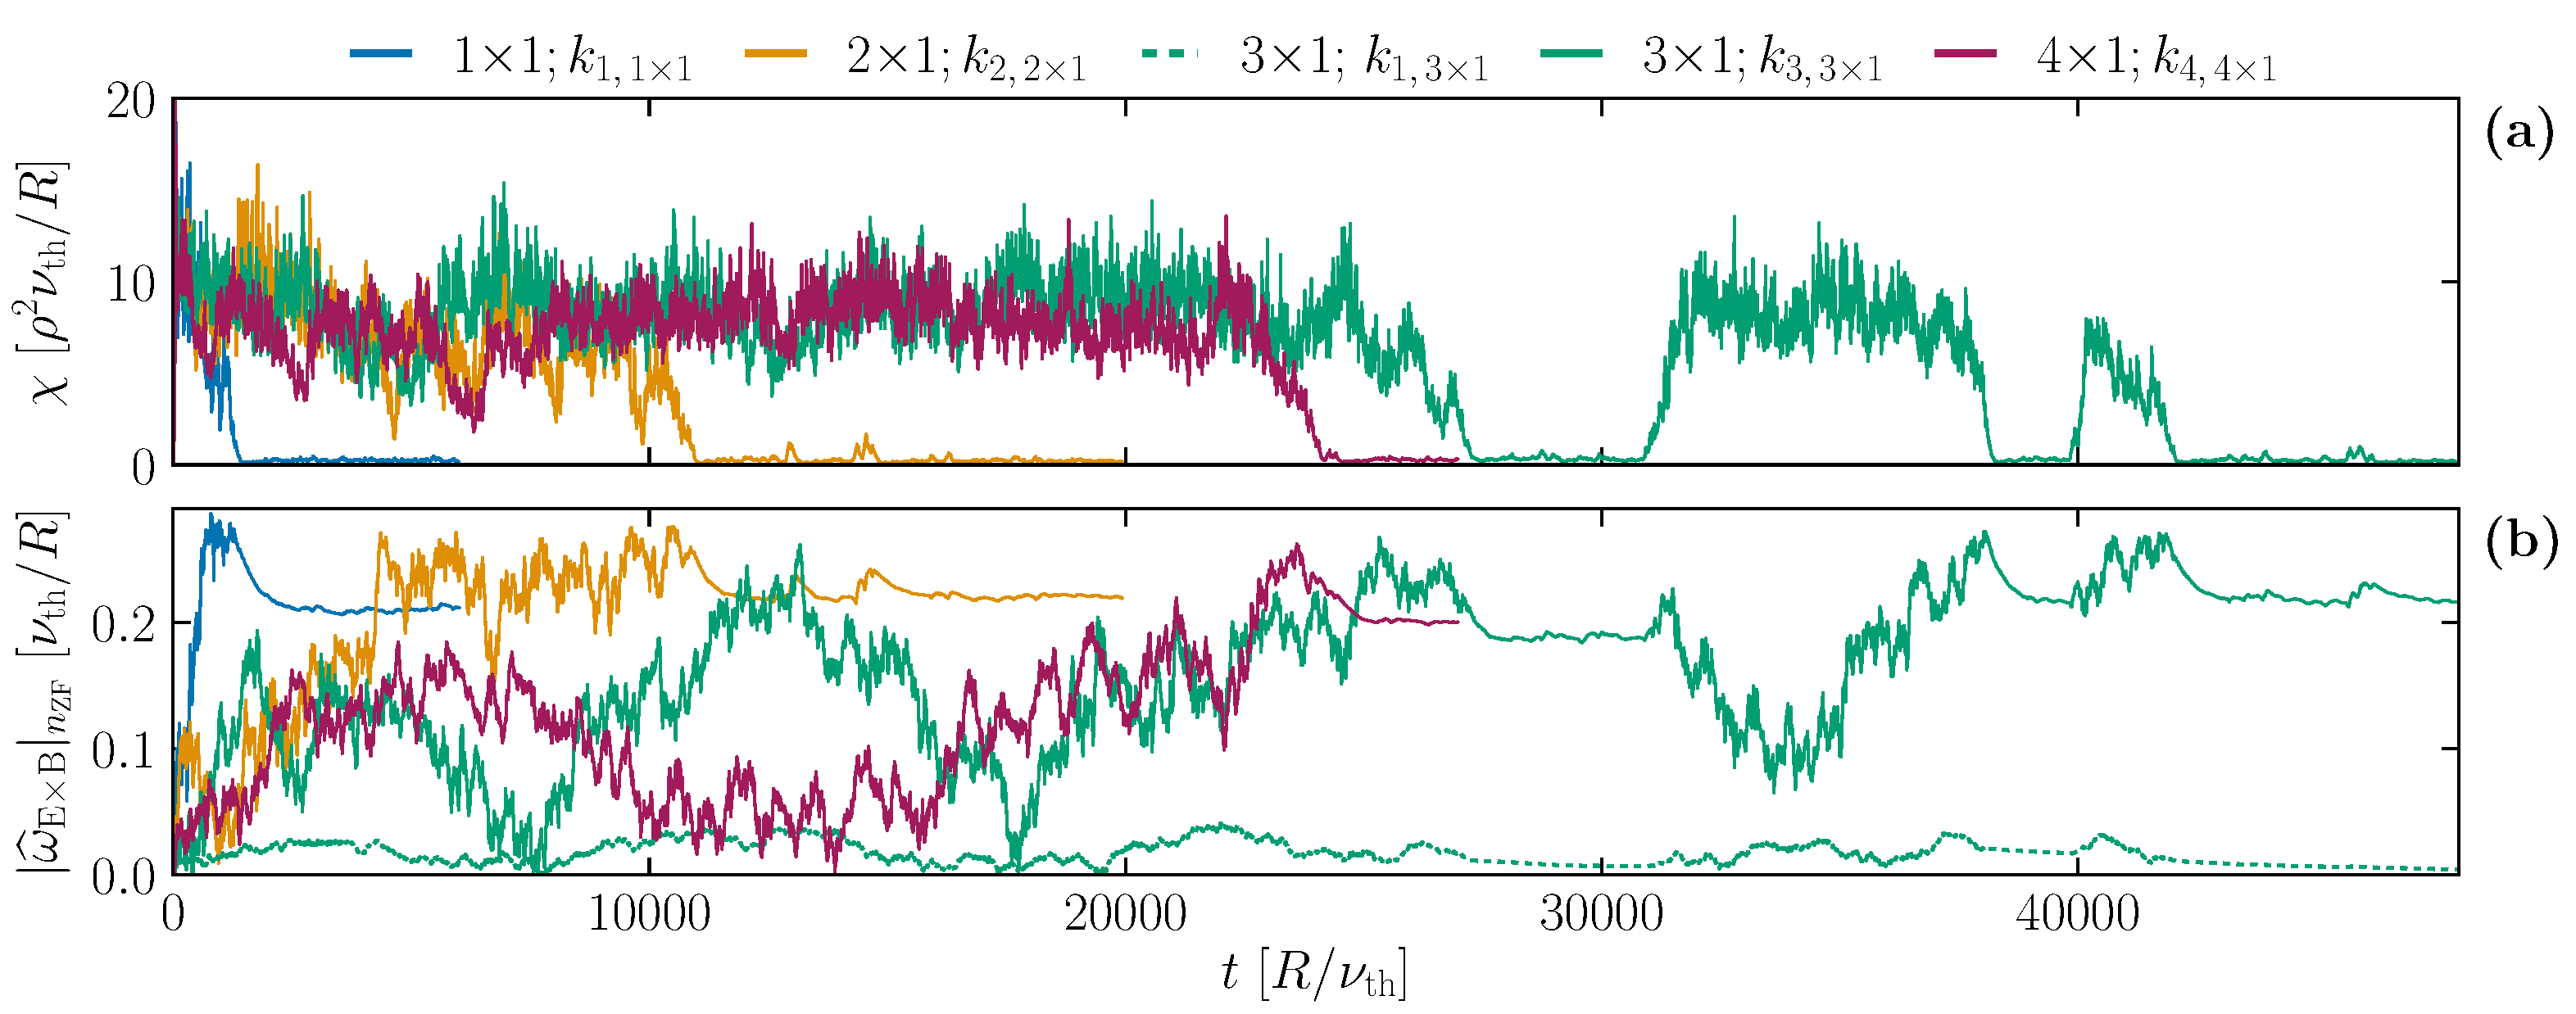
\includegraphics[width=0.\textwidth]{Briefcommunication/1.pdf}
	\captionof{figure}{
		\textbf{(a)} Time traces of the heat conduction coefficient $\chi$ for $\rlt = 6.0$ for radial increased box sizes,\\
		\textbf{(b)} Time traces of $\hatwexbamp$ for radial increased box sizes.
	}
	\label{fig:wexb-eflux-1-2-3-4x1-comparison}
\end{center}
\twocolumngrid

%% Include graphic for two column with specific place
\onecolumngrid
\begin{center}
	\centering
	\captionsetup{type=figure}
	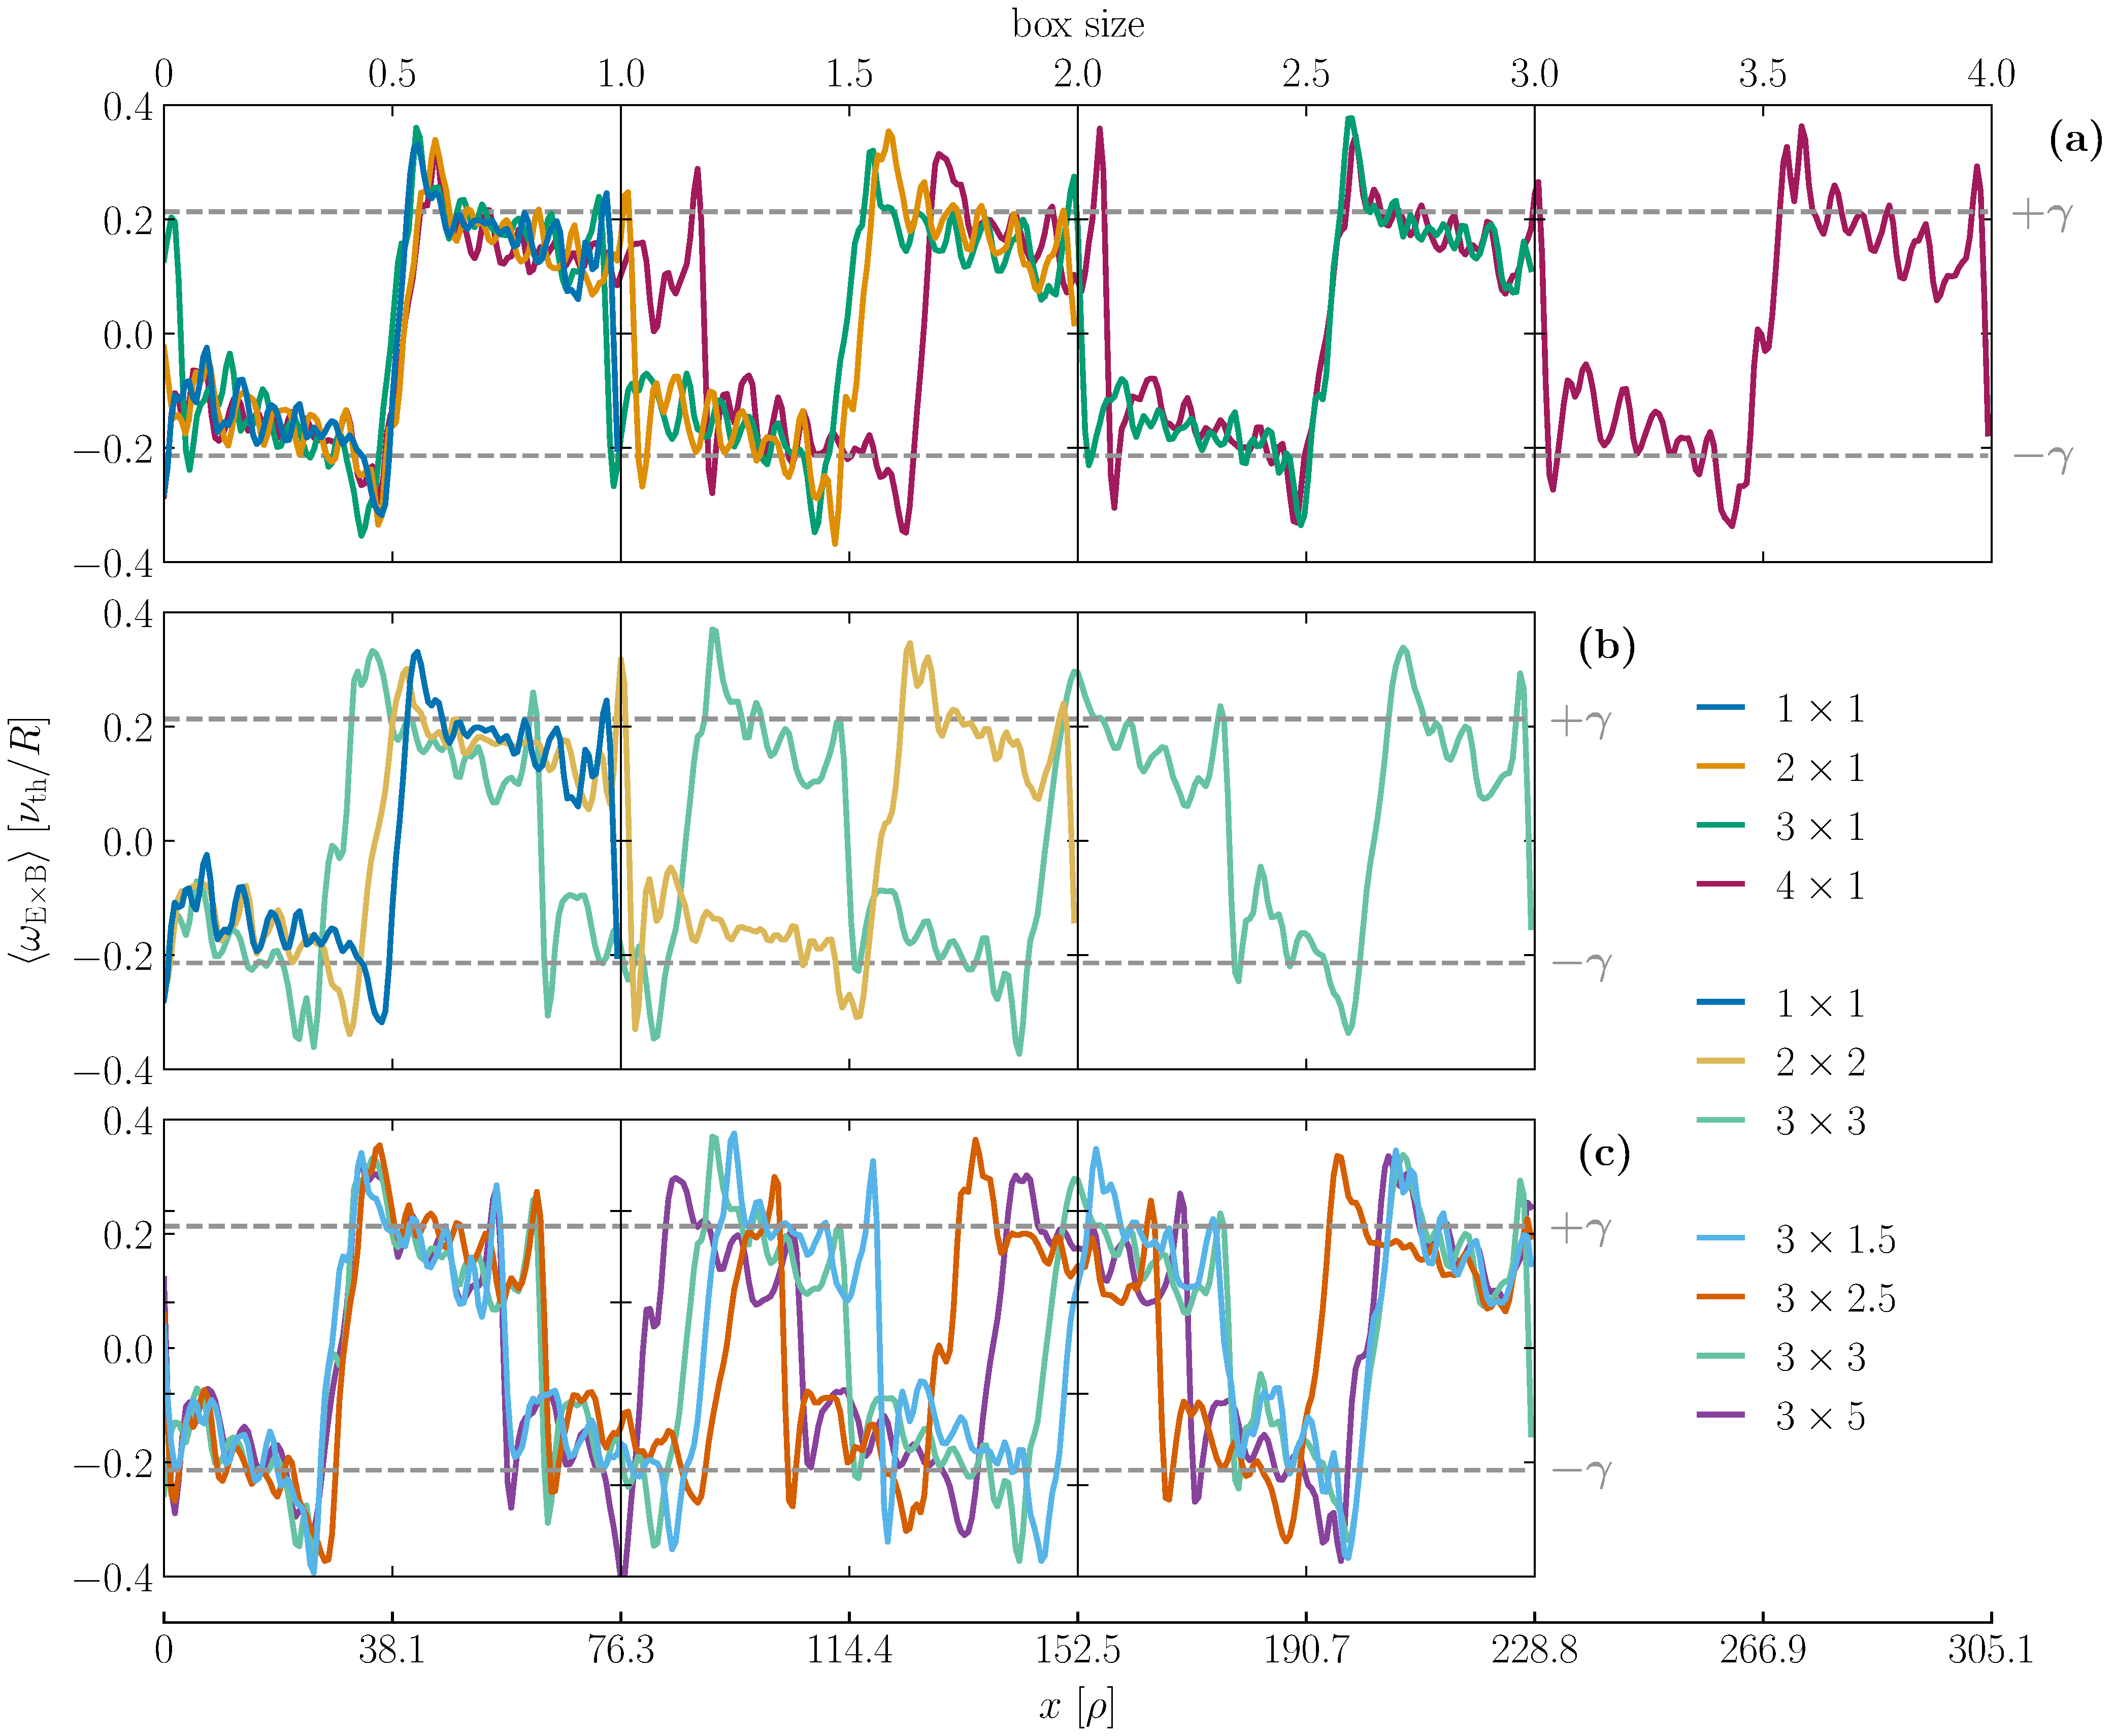
\includegraphics[width=0.98\textwidth]{Briefcommunication/2.pdf}
	\captionof{figure}{
		Comparison of shearing rate $\wexb$ for each box sizes scan averaged over given time interval and the growth rate $\pm \gamma$ of the most unstable linear ITG-driven Eigenmode. The staircase structures are radially shifted with respect to each over till alignment for better visibility:\\
		\begin{tabular}{l l l l l l l l l}
			\textbf{(a) radial:}    & $t_{1\times 1}$   & $\in [2000, 5000]$, & $t_{2\times 1}$   & $\in [15000, 18000]$, & $t_{3\times 1}$ & $\in [43000, 45000]$, & $t_{4\times 1}$ & $\in [26000, 28000]$;   \\
			\textbf{(b) isotropic:} & $t_{1\times 1}$   & $\in [2000, 5000]$, & $t_{2\times 2}$   & $\in [2000, 3000]$,   & $t_{3\times 3}$ & $\in [2000, 3000]$;   &                 &                         \\
			\textbf{(c) binormal:}  & $t_{3\times 1.5}$ & $\in [2000, 3000]$, & $t_{3\times 2.5}$ & $\in [2000, 3000]$,   & $t_{3\times 3}$ & $\in [2000, 3000]$,   & $t_{3\times 5}$ & $\in [1000, 3000]$.     \\
		\end{tabular}
	}
	\label{fig:wexb-stable-comparison}
\end{center}
\twocolumngrid

%% Include graphic for one column with specific place 
\begin{center}
	\centering
	\captionsetup{type=figure}
	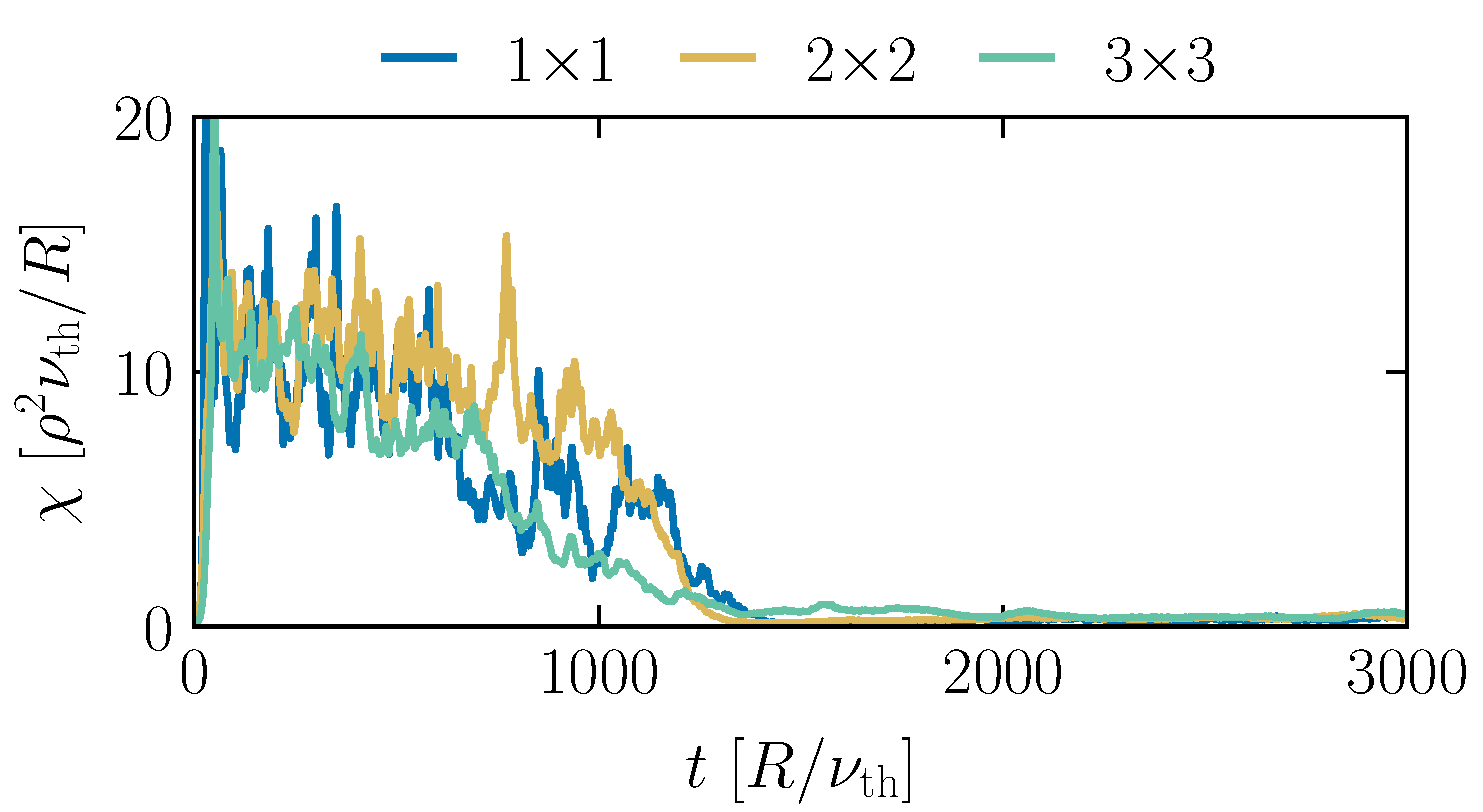
\includegraphics[width=0.87\linewidth]{Briefcommunication/3.pdf}
	\captionof{figure}{Time traces of the heat conduction coefficient $\chi$ for $\rlt = 6.0$ for isotropic increased box sizes.}
	\label{fig:eflux-1x1-2x2-3x3-comparison}
\end{center}

By contrast to the radial box size scan, the $3\times3$ realization shows a stationary pattern with four repetitions of the fully developed staircase structure, i.e., a somewhat smaller pattern size. 
Whether this is related to a possible pattern size dependence on the binormal box size or to the competition between patterns with the two sizes $\lambda \in [57,~ 76]\,\rhoth$ as observed in the first test is addressed in the next paragraph. 
The scale of structures developing in the $1.5\times1.5$ and $2.5\times2.5$ realizations (not included in Fig.~\ref{fig:wexb-stable-comparison} to preserve the clarity of this figure) also lie within the range given above.
Note that two additional realizations of the $3\times3$ case with different initial conditions and otherwise identical parameters confirm structure formation on scales within the range given above.\\

In a third test the binormal box size is varied with the radial box size fixed to $\NR = 3$.
This test covers the realizations $\NR \times \NB \in [3\times1.5,~3\times2.5,~3\times3,~3\times5]$. As in the isotropic scan the turbulence subdued and a fully developed staircase pattern forms after $\sim 2000\,R/\vth$ [Fig.~\ref{fig:eflux-3x1.5-2.5-3-5-comparison}]. The convergence of staircase pattern can be seen in Fig.~\ref{fig:wexb-stable-comparison}(c) and confirms again a size of a typical mesoscale. Fig.~\ref{fig:wexb-stable-comparison}(c) also confirms that indeed a competition between patterns with two sizes $\lambda \in [57,~ 76]\,\rhoth$ causing the different results for $3 \times 1$ and $3\times 3$. The zonal flow mode number varies between $\nzf = 3,4$ which can be seen in Fig.~\ref{fig:wexb-stable-comparison}(c) in the $3\times 2.5$ realization. The staircase structure has a pattern between three and four repetitions which get represented in the second repetition with no significant plateau at positive shear. Instead, the pattern returns immediately after reaching the maximum shear ($+ \gamma$) to the minimum shear ($- \gamma$) of the third repetition in a steep flank. The Fourier analysis of this case yields no definitely basic mode rather two dominating modes with $\nzf = 3, 4$ with a fraction of the maximum amplitude $\hatwexbamp$ each (not shown).

%% Include graphic for one column with specific place 
\begin{center}
	\centering
	\captionsetup{type=figure}
	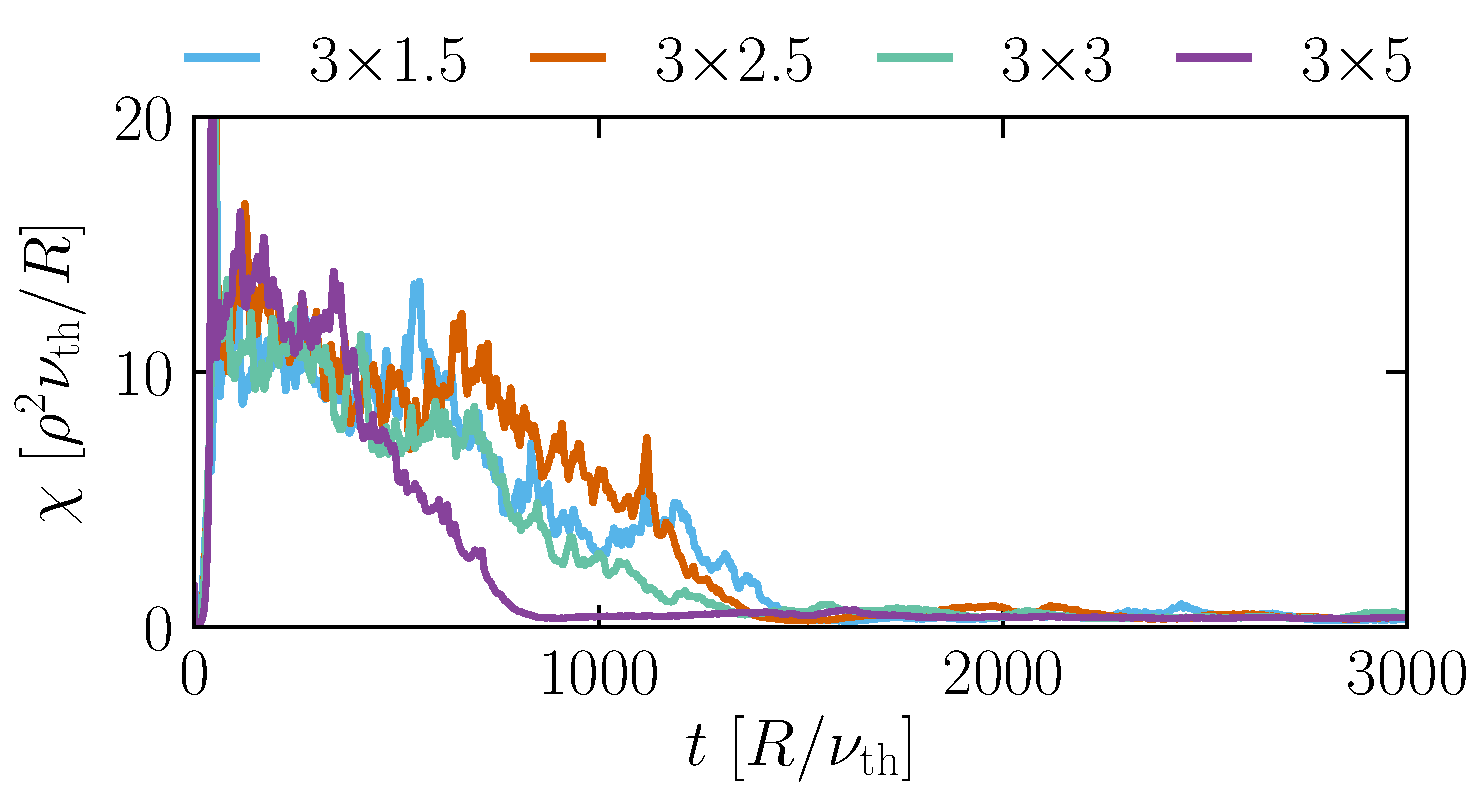
\includegraphics[width=0.87\linewidth]{Briefcommunication/4.pdf}
	\captionof{figure}{Time traces of the heat conduction coefficient $\chi$ for $\rlt = 6.0$ for binormal increased box sizes.}
	\label{fig:eflux-3x1.5-2.5-3-5-comparison}
\end{center}

In the final test the inverse background temperature gradient length $\rlt$ is varied at fixed $3\times3$ box size.
Since suppression of turbulence usually occurs at later times when approaching the finite heat flux threshold from below \cite{Peeters2016}, the analysis aims to lengthen the phase during which the zonal flow varies in time due to turbulent Reynolds stresses.
This scan covers realizations with $\rlt \in [6.0,~6.2,~6.4]$.
In the case of $\rlt = 6.2$ turbulence suppression is observed for $t > 11000\,R/\vth$, while stationary turbulence during the entire simulation time trace of $12000\,R/\vth$ is found for $\rlt = 6.4$.
The finite heat flux threshold, hence, is $\rlt|_\mathrm{finite} = 6.3 \pm 0.1$ in accordance with Ref. \onlinecite{Peeters2016}.
Although the initial quasi-stationary turbulence in the former case is significantly longer compared to the $\rlt = 6.2$ realization discussed in the second test, a stationary pattern with basic zonal flow mode $\nzf = 3$ establishes. 
Again, the $\nzf = 1$ (box scale) zonal flow mode does not grow secularly during the entire turbulent phase.
Also, this test confirms the statistical soundness of the converged pattern size of $\sim 57 - 76\,\rhoth$.\\ 


\bigskip

%%% CONCLUSION =============================================================================================================

Through careful tests this brief communication confirms the radial size convergence of the $\exb$ staircase pattern in local gyrokinetic flux tube simulations of ion temperature gradient (ITG)-driven turbulence.
A mesoscale pattern size of $\sim 57 - 76\,\rhoth$ is found to be intrinsic to ITG-driven turbulence for Cyclone Base Case parameters.
This length scale is somewhat larger compared to results from global studies with finite $\rho_\ast$, which report of a few $10\,\rhoth$ \cite{Pradalier2010}, and has to be considered the proper mesoscale in the local limit $\rho_\ast \rightarrow 0$.  
The occurrence of this mesoscale implies that non-locality, in terms of Ref. \onlinecite{Pradalier2010}, is inherent to ITG-driven turbulence, since avalanches are spatially organized by the $\exb$ staircase pattern \cite{McMillan2009, Pradalier2010, Rath2016, Peeters2016}. 

%% APPENDIX ================================================================================================================

\section*{Data Availability}
The data that support the findings of this study are available from the corresponding author upon reasonable request. 

% BIBLIOGRAPHY =============================================================================================================

\bibliography{references.bib}% Produces the bibliography via BibTeX.

\end{document}

% END MAIN =================================================================================================================
% ****** End of file aipsamp.tex ******